%%% CAPITOLO 5
%%% Capital Asset Pricin Model - CAPM - Valutazione del rischio
\section{Capital Asset Pricing Model - CAPM}

Il CAPM (\textbf{C}apital \textbf{A}sset \textbf{P}ricing \textbf{M}odel) è un modello che rappresenta la relazione tra 
i rendimenti aspettati di un indice rischioso ed il rischio di mercato (chiamato anche rischio sistematico).

Possiamo rappresentare il CAPM mediante la equazione:

\begin{displaymath}
    E(r_i) = r_f + \beta_i (E(r_m) - r_f)
\end{displaymath}

\textbf{dove}\\
\(E(r_i) = \text{Denota il rendimento aspettato dell'asset } i\)\\
\(r_f = \text{ratio risk-free}\)\\
\(E(r_m) = \text{Rendimento aspettato del mercato}\)\\
\(\beta = \text{coefficiente beta}\)

\subsection{Calcolo dell'indice beta}

L'indice beta si può interpretare come il livello di sensitività dei rendimenti di un asset relativamente al mercato.

\begin{itemize}
    \item \(\text{beta} \le -1\): L'asset si muove nella direzione opposta al benchmark e in un ammontare superiore rispetto al negativo del benchmark.
    \item \(-1 < \text{beta} < 0\): L'asset si muove nella direzione opposta al benchmark.
    \item \(\text{beta} = 0\): Non esiste correlazione tra il movimento del prezzo dell'asset e il benchmark di mercato.
    \item \(0 < \text{beta} < 1\): L'asset si muove nella stessa direzione del mercato, ma con un ammontare inferiore. (per esempio uno stock di una compagnia che non è molto suscettibile a fluttuazioni giornaliere).
    \item \(\text{beta} = 1\): L'asset ed il mercato si muovono nella stessa direzione e con lo stesso ammontare.
    \item \(\text{beta} \ge 1\): L'asset si muove nella stessa direzione del mercato, ma l'ammontare è maggiore (per esempio nel caso di stock che sono molto suscettibili a cambiamenti giornalieri nelle notizie di mercato). 
\end{itemize}

La equazione del CAPM può essere modificata per ottenere la formula di calcolo per beta

\begin{displaymath}
    \beta = \frac{cov(R_i,R_m)}{var(R_m)}
\end{displaymath}

Nel calcolo di beta per tutti i titoli considerati in questo progetto verrà considerato l'indice \verb|S&P 500| (\verb|^GSPC|).

Mediante il metodo delle covarianze l'indice beta per ogni titolo è:
\begin{itemize}
    \item Meta (FB): $1.1146$
    \item Alphabet (GOOG): $1.0138$
    \item Raytheon (RTX): $1.3118$
    \item Lockheed Martin(LMT): $0.835$
    \item Bank of America(BAC): $1.5124$
    \item JPMorgan Chase (JPM): $1.2579$
\end{itemize}

\pagebreak

\subsection{Calcolo esposizione dei titoli con Fama-French}

Il modello a tre fattori Fama-French è stato inventato per espandere il modello CAPM aggiungendo due fattori
che aiutano a spiegare l'eccesso di ritorno di un asset o portfolio. I tre fattori considerati sono:
\begin{itemize}
    \item \textbf{Market Factor (MKT)}: Misura l'eccesso di ritorno del mercato, uguale a quello che troviamo nel CAPM.
    \item \textbf{Size factor, SMB(Small Minus Big)}: Misura l'eccesso di ritorno degli stock con un market cap piccolo rispetto agli stock con un grande market cap.
    \item \textbf{Value factor, HML(High Minus Low)}: Misura l'eccesso di ritorno dei \verb|value stock| rispetto ai \verb|growth stock|.
    I \verb|value stock| hanno un alto ratio book-to-market, mentre i \verb|growth stock| sono caratterizzati da un basso ratio.
\end{itemize}

Possiamo rappresentare il modello come

\begin{displaymath}
    E(r_i) - r_f = \alpha + \beta_{mkt}MKT + \beta_{smb}SMB + \beta_{hml}HML
\end{displaymath}

\textbf{dove}\\
\(E(r_i) = \text{Denota il rendimento aspettato dell'asset } i\)\\
\(r_f = \text{ratio risk-free}\)\\
\(\alpha = \text{costante di intercettamento (equivalente a 0)}\)

Per l'utilizzo di questo modello in questo progetto sono stati scaricati i dati direttamente dal sito del Professor 
French\footnote{
    \href{http://mba.tuck.dartmouth.edu/pages/faculty/ken.french/ftp/F-F_Research_Data_Factors_CSV.zip}{http://mba.tuck.dartmouth.edu/pages/faculty/ken.french/ftp/F-F\_Research\_Data\_Factors\_CSV.zip}
}.

\subsubsection{Esposizione di Meta (FB)}

\begin{figure}[ht]
    \centering
    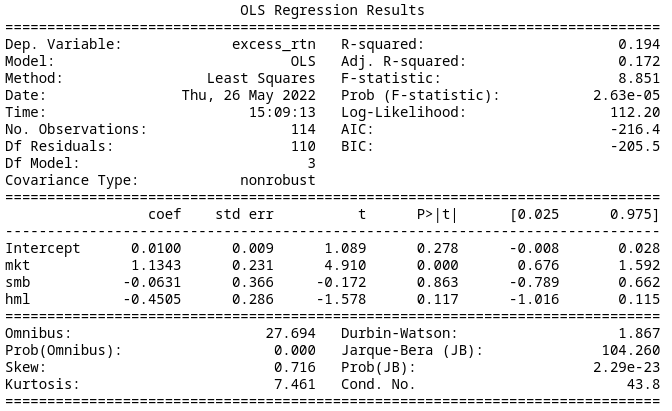
\includegraphics[width=0.75\textwidth]{fb_fama_french.png}
    \caption{Risultati del modello Fama-French per FB}
    \label{fig:fb_fama_french}
\end{figure}

Dai risultati del modello Fama-French a figura \ref{fig:fb_fama_french} troviamo come fattore \verb|SMB| $-0.0631$ e come fattore \verb|HML| il valore $-0.4505$, l'intercept non presenta un valore significante.

\pagebreak

\subsubsection{Esposizione di Alphabet (GOOG)}

\begin{figure}[ht]
    \centering
    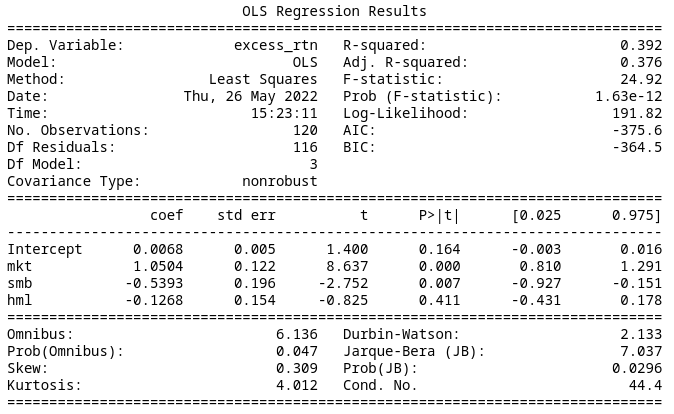
\includegraphics[width=0.75\textwidth]{goog_fama_french.png}
    \caption{Risultati del modello Fama-French per GOOG}
    \label{fig:goog_fama_french}
\end{figure}

Dai risultati del modello Fama-French a figura \ref{fig:goog_fama_french} troviamo come fattore \verb|SMB| $-0.504$ e come fattore \verb|HML| il valore $-0.1268$, 
anche in questo caso l'intercept non presenta un valore significante.

\subsubsection{Esposizione di Raytheon (RTX)}

\begin{figure}[ht]
    \centering
    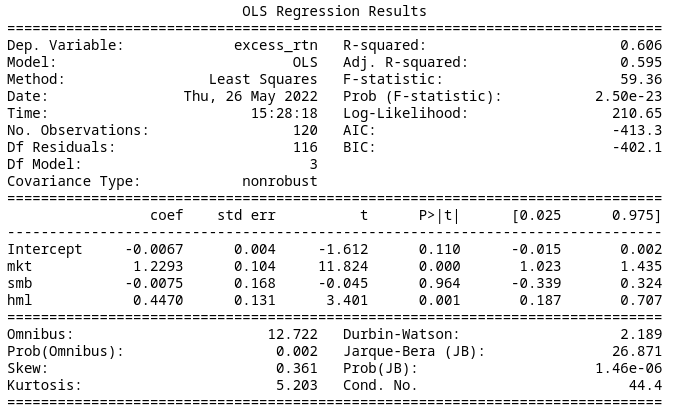
\includegraphics[width=0.75\textwidth]{rtx_fama_french.png}
    \caption{Risultati del modello Fama-French per RTX}
    \label{fig:rtx_fama_french}
\end{figure}

Dai risultati del modello Fama-French a figura \ref{fig:rtx_fama_french} troviamo come fattore \verb|SMB| $-0.0075$ e come fattore \verb|HML| il valore $0.4470$, 
in questo caso l'intercept non presenta un valore significante.

\pagebreak

\subsubsection{Esposizione di Lockheed Martin (LMT)}

\begin{figure}[ht]
    \centering
    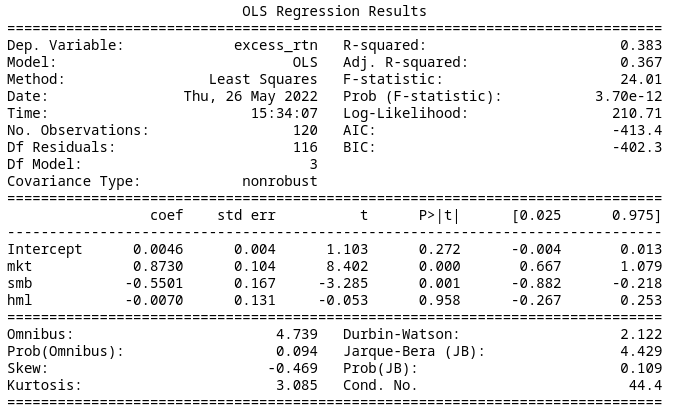
\includegraphics[width=0.75\textwidth]{lmt_fama_french.png}
    \caption{Risultati del modello Fama-French per LMT}
    \label{fig:lmt_fama_french}
\end{figure}

Dai risultati del modello Fama-French a figura \ref{fig:lmt_fama_french} troviamo come fattore \verb|SMB| $-0.5501$ e come fattore \verb|HML| il valore $-0.0070$, 
in questo caso l'intercept non presenta un valore significante.

\subsubsection{Esposizione di Bank of America (BAC)}

\begin{figure}[ht]
    \centering
    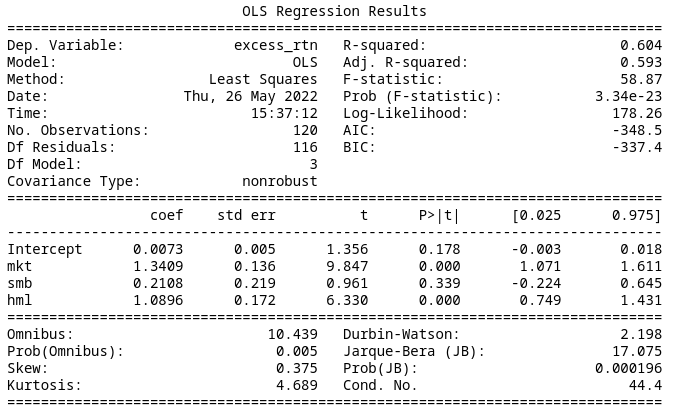
\includegraphics[width=0.75\textwidth]{bac_fama_french.png}
    \caption{Risultati del modello Fama-French per BAC}
    \label{fig:bac_fama_french}
\end{figure}

Dai risultati del modello Fama-French a figura \ref{fig:bac_fama_french} troviamo come fattore \verb|SMB| $0.2108$ e come fattore \verb|HML| il valore $1.0896$, 
in questo caso l'intercept non presenta un valore significante mentre invece il valore \verb|HML| supera $1$.

\pagebreak

\subsubsection{Esposizione di JPMorgan Chase (JPM)}

\begin{figure}[ht]
    \centering
    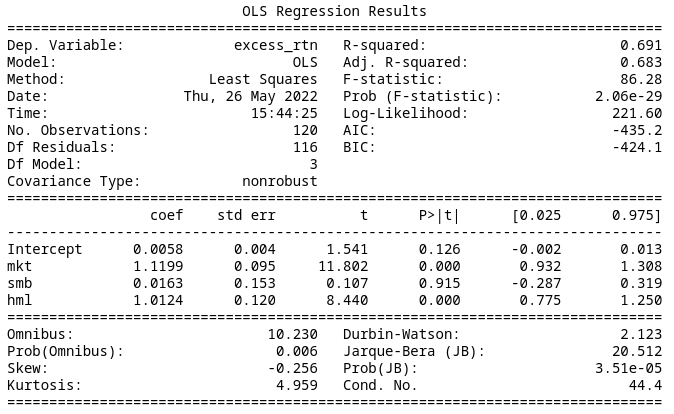
\includegraphics[width=0.75\textwidth]{jpm_fama_french.png}
    \caption{Risultati del modello Fama-French per JPM}
    \label{fig:jpm_fama_french}
\end{figure}

Dai risultati del modello Fama-French a figura \ref{fig:jpm_fama_french} troviamo come fattore \verb|SMB| $0.0163$ e come fattore \verb|HML| il valore $1.0124$, 
in questo caso l'intercept non presenta un valore significante mentre invece il valore \verb|HML| come per BAC supera $1$.